
%\section{Биография}
%\sectionmark{Биография}

Этот вид занесен в Красную книгу Международного союза охраны природы.

Европейская болотная черепаха распространена в местах умеренного климата. Проживает в Центральной и Южной Европе, Передней Азии, Америке,Западной Европе, Северно-Западной Африки. В России распространена в теплой зоне умеренного климата европейской части.

Проживает черепаха на медленно протекающих реках, прудах, озерах с пологими берегами и илистым дном.
Впадают в спячку болотные черепахи осенью, в октябре, тем самым пережидают зиму на дне водоемов.

\begin{figure}[H]
  \center{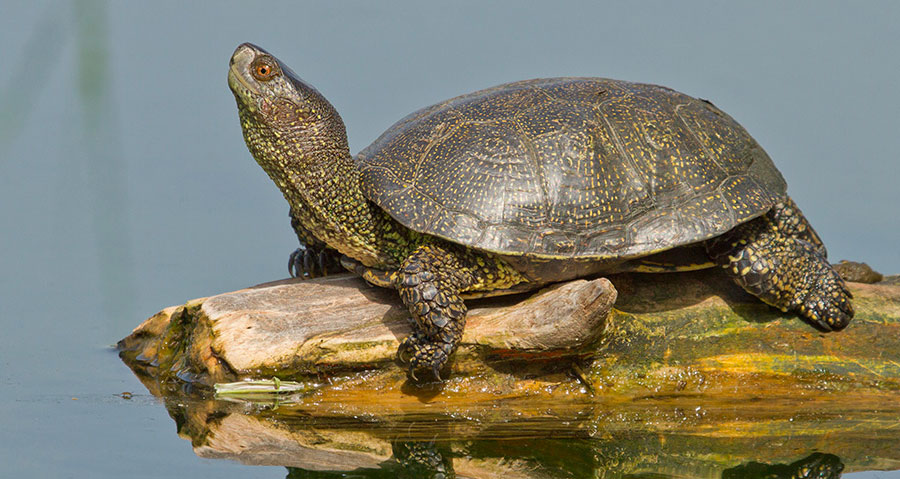
\includegraphics[width=0.6\textwidth]{./src/3-1.jpg}}
%  \caption{} \label{p:1}
\end{figure}

В зависимости от подвида длина панциря доходит до 18–25 см, а самцы как правило меньше самок. В природе проживают до 120 лет.

Болотная черепаха в ночное время спит на дне водоема ,а в дневные часы сохраняет активность . Коротает по нескольку часов под лучами солнца на суше . Может удаляться на несколько километров от водоемов. Болотная черепаха плавает очень быстро , зарывается в ил при даже мизерной угрозе, и довольно стремительно передвигается по земле. 


В естественной природе главными источниками питания являются мелкие лягушки, рыба, мокрицы, личинки насекомых, червяки, моллюски, прибрежные и водные растения.

\begin{figure}[H]
  \center{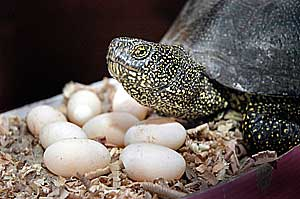
\includegraphics[width=0.6\textwidth]{./src/Cherepaha_1.jpg}}
%  \caption{} \label{p:1}
\end{figure}


В естественных условиях самки черепах откладывают около 5-12 яиц в период с мая по июль. За это время самка осуществляет 1-3 кладки (как правило в мае, июне и июле). Яйца болотных черепах овальные, покрытые жесткой скорлупой, длиной около 28-33 миллиметров и шириной около 18-20 миллиметров, весом примерно 8 г. Откладывают самки яйца в ночное время в первоначально выкопанные ямки глубиной около 10-12 см. Маленькие черепахи длинной примерно 15 миллиметров вылупливаются через 2-3 месяца в период с августа по октябрь. Первую зиму они проводят в земле, питаются за счет желточного мешка, находящегося в брюшных щитках пластрона. Появляются из земли , как правило ,только лишь к следующей весне.

Природных врагов у болотной черепахи немного. И те грозят в основном новорождённым, чей панцирь ещё недостаточно окреп и не может защитить от когтей и зубов хищников. Главную опасность для них представляет именно человек: он не только отлавливает черепах, но и уничтожает их естественную среду обитания, осушая болота и водоёмы.





















